\documentclass{standalone}
\usepackage{tikz}
\usetikzlibrary{patterns}

\tikzset{
  svgfrag/.style 2 args={
    execute at begin scope={\special{dvisvgm:raw <g class="fragment #2" data-fragment-index="#1">}},
    execute at end scope={\special{dvisvgm:raw </g>}},
    execute at begin node={\special{dvisvgm:raw <g class="fragment #2" data-fragment-index="#1">}},
    execute at end node={\special{dvisvgm:raw </g>}},
  }
}

\begin{document}
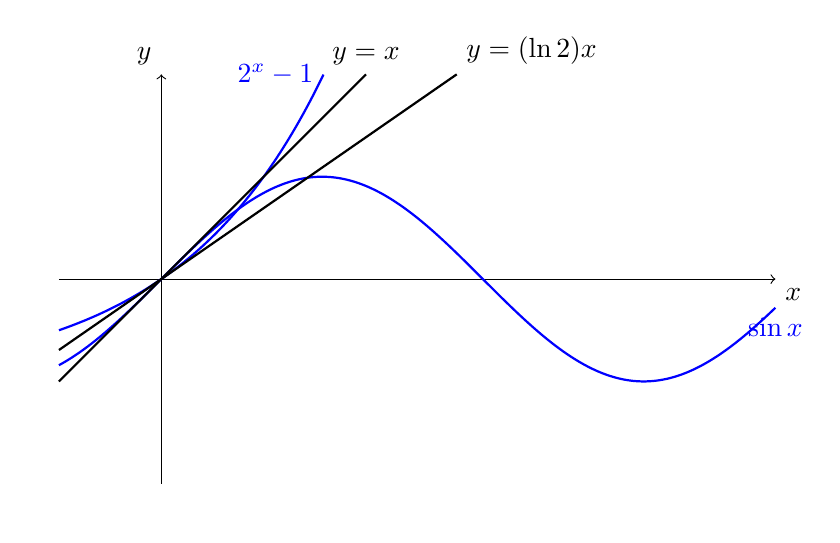
\begin{tikzpicture}[scale=1.3]
    \draw[white] (-1.3,-2.3) rectangle (6.3,2.3);
    \draw[thin, ->] (-1,0) -- (6,0)node[below right]{$x$};
    \draw[thin, ->] (0, -2) -- (0, 2)node[above left]{$y$};
    \draw[thick, domain=-1:6, blue] plot[samples=200] (\x, {sin(\x r)})node[below]{$\sin x$};
    \draw[thick, domain=-1:1.585, blue] plot[samples=200] (\x, {exp(\x*ln(2)) - 1})node[left]{$2^x - 1$};
    \begin{scope}[svgfrag={1}{fade-in}]
        \draw[thick] (-1,-1) -- (2,2);
    \end{scope}
    \begin{scope}[svgfrag={2}{fade-in}]
        \node[above] at (2,2) {$y = x$};
    \end{scope}
    \begin{scope}[svgfrag={3}{fade-in}]
        \draw[thick] (-1,-0.693) -- (2.886,2);
    \end{scope}
    \begin{scope}[svgfrag={4}{fade-in}]
        \node[above right] at (2.886,2) {$y = (\ln 2)x$};
    \end{scope}
\end{tikzpicture}
\end{document}
